\documentclass{article}

\usepackage[utf8]{inputenc}
\usepackage[T1]{fontenc}
\usepackage[french]{babel}
\usepackage{tabularx}
\usepackage{graphicx}

\title{Module TLC
\\
--
\\
Google App Engine}
\author{Thibaud Destouches - Lacroix Marceau}
\date{2012 - 2013}

\begin{document}

\begin{titlepage}
\maketitle
\tableofcontents
\end{titlepage}

\newpage
\section{Introduction}

Le but de ce TP est d’aborder le développement d'application pour le Google App Engine, nous allons donc créer une plateforme de publicité simple, avec des fonctionnalités simples telles que la création, la suppression, ou encore la recherche de publicité.

\section{Implémentation}
Avant de déployer notre application sur le Google App Engine, nous avons téléchager le SDK permettant de tester nos applications localement, cela permet ainsi un gain de temps conséquant pendant le développement.

Nous avons fait le choix de programmer cette application en J2EE, en effet il est uniquement possible de développer pour le Google App Engine en Python ou en J2EE. Nous nous sommes donc basé sur des fichiers JSP pour la mise en forme, et avons implémenter des services qui s'occupent d'effectuer les opérations sur la base de données.

\section{Mesure de performance}
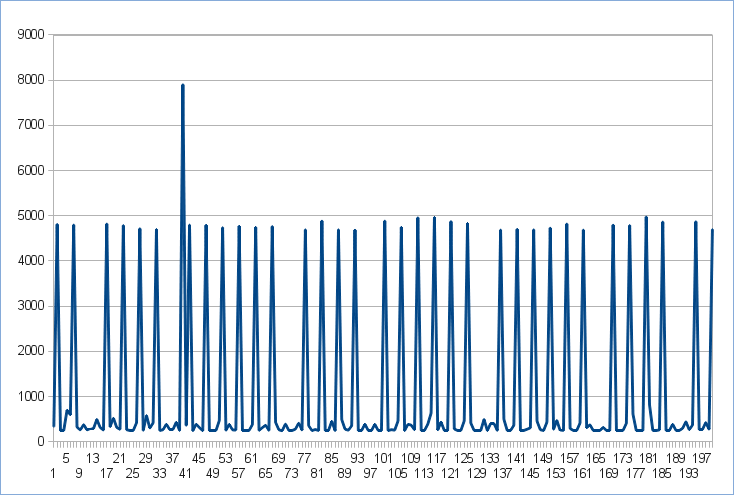
\includegraphics[scale=0.5]{measure}

On distingue sur ce graphique des pics de "lenteur" en effet toutes les 10 requetes la suivante prend environ 5 secondes alors que les autres requêtes s'exécutent en moins de 0,5 seconde. Rien que cette "limite" que nous percevons dès les premiers tests nous donne un à priori plutôt négatif sur la technologie GAE.

\section{Difficultées}
La principale difficulté que nous avons rencontré est l'usage de JPA pour la gestion de la persistance. En effet, le Google App Engine n'implémente pas la totalité de la librairie JPA, nous contraignant ainsi à développer nos fonctionnalités différemment de si nous avions eu à le faire pour une servlet "classique". 

D'autre part, la fonction de recherche nous à aussi posé pas mal de problèmes. Nous avons commencé par l'implementer "à la main", c'est à dire en faisant une requête relativement large et en triant les résultats \footnote{en leur attribuant un score en fonction des critères de recherche}. Nous avons ensuite découvert la librairie "search" que fournit google pour app engine. Cette API est relativement complexe à prendre en main mais semble fournir de bons résultats et permet de faire des requetes multiples relativement facilement. De plus on à accès à la "syntaxe google" pour les requêtes; on peut par exempl entrer "foo OR bar" pour obtenir les annonces dont le titre est foo ou bar. Nous n'avons malheureusement pas trouvé le "joker"\footnote{On ne peut donc pas trouver "foobar" en cherchant "foo", "bar", "foo OR bar" mais uniquement en cherchant exactement "foobar".}.


\section{Conclusion}
Grâce à ce TP nous avons pu constater la puissance du Google App Engine, en effet le fait de complètement s'abstraire de l'infrastructure sur laquelle est exécutée l'application permet de se concentrer sur le développement de celle-ci sans avoir à gérer tous les soucis innérent à la gestion d'un serveur. Mais nous avons pu également observer les limites de ce système, le support uniquement des langages Python et J2EE bride fortement la possibilité de développement sur cette plateforme, de plus la limitation même des librairies utilisables sur le Google App Engine empêche souvent le développeur de faire ce qu'il veut et doit donc se limiter à ce qui lui est fourni par Google.

Pour conclure, nous pensons que Google App Engine n'est pas un mauvais système, mais qu'il doit se limiter aux petites infrastructure qui ont uniquement un besoin limité et ne souhaite pas passer du temps à installer et maintenir un serveur. Pour tous les autres, Google App Engine n'est pas a conseillé.


\end{document}
